\documentclass[
	article,			
	11pt,				
	oneside,			
	a4paper,			
	english,			
	brazil,				
	sumario=tradicional
	]{abntex2}

\usepackage{lmodern}			
\usepackage[T1]{fontenc}		
\usepackage[utf8]{inputenc}		
\usepackage{indentfirst}		
\usepackage{nomencl} 			
\usepackage{color}			
\usepackage{graphicx}			
\usepackage{microtype} 			
\usepackage{lipsum}			
\usepackage[brazilian,hyperpageref]{backref}
\usepackage[alf]{abntex2cite}
\newenvironment{myfont}{\fontfamily{pcr}\selectfont}{\par}

\renewcommand{\backrefpagesname}{Citado na(s) página(s):~}
\renewcommand{\backref}{}
\renewcommand*{\backrefalt}[4]{
	\ifcase #1 %
		Nenhuma citação no texto.%
	\or
		Citado na página #2.%
	\else
		Citado #1 vezes nas páginas #2.%
	\fi}%

\titulo{O uso do algoritmo LZ78 na urna eletrônica}
\autor{Raphael Rodrigues Pereira (1822130030)}
\local{Brasil}
\data{Novembro de 2018}
\definecolor{blue}{RGB}{41,5,195}

\makeatletter
\hypersetup{
     	%pagebackref=true,
		pdftitle={\@title}, 
		pdfauthor={\@author},
    	pdfsubject={LZ78 para urnas eletrônicas},
	    pdfcreator={Raphael Rodrigues},
		pdfkeywords={urna}{lz78}, 
		colorlinks=true,       		% false: boxed links; true: colored links
    	linkcolor=blue,          	% color of internal links
    	citecolor=blue,        		% color of links to bibliography
    	filecolor=magenta,      		% color of file links
		urlcolor=blue,
		bookmarksdepth=4
}
\makeatother
\makeindex
\setlrmarginsandblock{3cm}{3cm}{*}
\setulmarginsandblock{3cm}{3cm}{*}
\checkandfixthelayout

\setlength{\parindent}{1.3cm}
\setlength{\parskip}{0.2cm}
\SingleSpacing

\begin{document}

\selectlanguage{brazil}

\frenchspacing 

\twocolumn[    		% INICIO DE ARTIGO EM DUAS COLUNAS
\maketitle

\begin{resumoumacoluna}
Com uma crescente necessidade de colocar uma maior quantidade de arquivos no disco, sendo estes com uma grande quantidade de dados, houve uma preocupação em diminuir o tamanho dos arquivos armazenados, a fim de que ocupassem menos espaço na memória secundária. Sendo assim, foi-se pensado nos algoritmos de compressão de dados, que procura solucionar essa problemática. Neste trabalho verificar-se-á que o algoritmos, tais como o de Lempel-Ziv, de 1978, utilizado amplamente nos dias de hoje. podem comprimir os arquivos em até 52,52\% do seu tamanho original, para formato TXT e até 83,20\% para formato binário, mostrando uma melhor performance em relação ao algorimo LZ77.
 
 \vspace{\onelineskip}
 
 \noindent
 \textbf{Palavras-chave}: LZ78, urna eletrônica, algoritmo, compressão, tempo de execução.
\end{resumoumacoluna}

]  				% FIM DE ARTIGO EM DUAS COLUNAS

\textual

\section*{Introdução}
\addcontentsline{toc}{section}{Introdução}
Na década de 20, com o crescimento da população brasileira, o número de votos aumentou consideravelmente, de modo que fosse necessário um sistema mais ágil para a contabilização dos votos eleitorais. Sendo assim, desde 1989 até os dias atuais a implantação da urna eletrônica tem sido um sucesso, diminuindo, com o avanço da tecnologia, cada vez mais o tempo de apuração dos votos eletrônicos. Mas, no decorrer dos anos de implantação da nova tecnologia, surgiram alguns problemas em sua composição, como por exemplo uma maior segurança no seu sistema, para prevenir fraudes e roubo de informações, houve uma demanda por um sistema mais rápido e consistente, que não apresentasse problemas computacionais, como também uma necessidade de se carregar os votos da urna para um dispositivo externo. A partir disso, a compressão de dados foi vista como uma ferramenta essencial para a integridade e velocidade da urna eletrônica. Neste artigo será utilizado o algoritmo de Lempel-Ziv, criado em 1978, denominado LZ78, para realizar a compressão dos dados de modo que seja possível um melhor transporte e armazenamento dos votos eletrônicos. Sendo assim, serão feitas compactações de arquivos binários e arquivos texto para a comparação em relação à velocidade de execução e ao tamanho ocupado em disco.

\section{Problemática}
A computação dos votos a partir de uma urna eletrônica gera uma alta densidade de dados, devido ao fato de que os votos computados somam em 147.302.357 \cite{eleitores2018}, de acordo com o TSE (Tribunal Superior Eleitoral). Sendo assim, serão gigas de dados a serem armazenados para serem apurados posteriormente. Deste modo, o transporte dos dados seria mais complexo, demandando mais tempo para a sua transferência, aumentando, assim, o tempo de espera para o resultado das eleições. Visto isso, desenvolvemos um modelo do algoritmo LZ78, desenvolvido em 1978 pela dupla Abraham Lempel e Jacob Ziv \cite{christinazeeh2013}.
A escolha deste algoritmo e não do LZ77, verão anterior a ele, se dá principalmente por conta do estudo de ZEEH \cite{christinazeeh2013}, que mostrou que os algoritmos da família do LZ78 são mais rápidas e mais compactos em relação aos algoritmos da família do LZ77, como na imagem a seguir: 
\begin{center}
	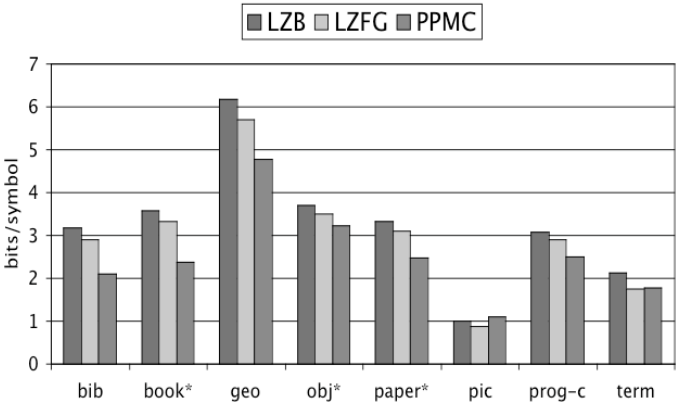
\includegraphics[width=7cm,height=4cm]{LZ77_LZ78.png}\\
	Imagem 1 - Taxa de compressão x Tempo de execução para arquivo binário.
\end{center}

\section{Funcionamento do LZ78}
O algoritmo implementado utiliza um dicionário estático, que servirá para armazenar os dados compactados \cite{jziv1977}. Este arquivo é composto de uma dupla (X,Y), em que X representa o índice da maior palavra e Y corresponde ao último caracter que será inserido. Por exemplo, ao entrar-se com a palavra "wabba wabba". Inicialmente o algoritmo verificará no dicionário a existência da dupla, mas ele não contém nenhuma dupla no momento. Sendo assim, ele irá adicionar no dicionário a dupla (0,w) na linha 1. Para o segundo caracter lido, a letra "a", o algoritmo verificará se existe a dupla (0,a) no dicionário, passando pela primeira linha inserida anteriormente, e inserindo a dupla no final do arquivo, na linha 2. O mesmo procedimento será aplicado ao ler o caracter "b" da string, colocando (0,b) na terceira linha. Agora, ao ler o segundo "b" da palavra o procedimento será um pouco diferente, ele irá verificar se já existe a dupla (0,b) no dicionário. Como já existe, ele armazenará a linha da ocorrência achada e lerá o caracter seguinte ao "b" lido, neste caso o "a". Assim, ele analisará, neste momento, se existe a dupla (3,a) no dicionário. Como não existe, ele criará na última linha do arquivo, a linha 4. E assim, por diante até que se chegue no final da string. No últim elemento, caso necessário, deverá deixar seu índice sem o próximo caracter, ficando uma dupla da seguinte maneira (INDICE,""). Seu funcionamento completo está representado na tabela a seguir. 

\begin{table}[h!]
  \begin{center}
    \label{tab:table1}
     \begin{tabular}{c|c|c} % <-- Alignments: 1st column left, 2nd middle and 3rd right, with vertical lines in between
      \textbf{Índice} & \textbf{Caracter} & \textbf{Dicionário}\\
      \hline
      1 & w & (0,w)\\
      2 & a & (0,a)\\
      3 & b & (0,b)\\
      4 & ba & (3,a)\\
      5 & \textbackslash s & (0,\textbackslash s)\\
      6 & wa & (1,a)\\
      7 & bb & (3,b)\\
      8 & a & (2,)\\
    \end{tabular}
    \caption{Compressão da string wabba wabba.}
  \end{center}
\end{table}

Para a descompactação foi necessário fazer o procedimento oposto ao da compactação, em que, ao ler uma entrada no dicionário, é necessário armazenar o valor lido em um arquivo texto, caso seja índice zero. Caso o índice seja diferente de zero, será criado um outro arquivo que funcionará como um auxiliar para a palavra lida. Por exemplo, se o loop ler, no exemplo anterior, o (3,a), ele irá salvar o caracter "a" nesse arquivo auxiliar e irá para a linha 3, que corresponde ao índice do caracter anterior ao "a" da string, ou seja, será necessário "pular" para o índice lido do arquivo de dicionário para que seja possível criar a string original, sendo assim, ele irá para a linha 3 do arquivo de dicionário, pegando o caracter b, armazenando também no arquivo auxiliar. Após, foi criada uma pilha para ler o arquivo auxiliar, printando no arquivo de saída o inverso da string contida no arquivo auxiliar, para que saia no formato correto. 

\section{Ambiente}

A implementação do algoritmo bem como os testes executados foram realizados através de uma máquina rodando o sistema operacional Ubuntu, versão 14.04.1. Para a compilação da urna eletrônica e do algoritmo de compressão de dados foram utilizados o compilador GCC, versão 4.9.4, em que ambos códigos foram escritos em linguagem de programação C. Para a conversão de um arquivo texto para um arquivo binário, a conversão do arquivo contendo os candidatos a distrital e regional do TSE para o desejado e para a conversão de um arquivo UTF-8 para ASCII, foram utilizados o Python 2.7.6.

\section{Procedimentos}

Para a programação da urna eletrônica foi necessário saber o seu funcionamento básico, o voto eletrônico. Para isso, foi feita uma votação pedindo ao usuário que digitasse o seu CPF, passando pela validação oficial do TSE e o número do candidato que ele deseja votar. Após a entrada do número do candidato, há uma confirmação se o candidato digitado é de fato o candidato desejado pelo usuário, mostrando o nome do candidato e o seu respectivo partido, como no exemplo: \\
\newline
\begin{myfont}
{\footnotesize PARTIDO = PRB}\\
{\footnotesize CANDIDATO = GEORGE ARTHUR MOTTA DE SOUZA}\\
{\footnotesize NUMERO = 10010}\\
\end{myfont}

Outras opções que também o usuário pode escolher na urna eletrônica são as:
\begin{itemize}
\item Buscar um candidato por estado (DF, GO, MS), que são os estados que são abordados neste trabalho.
\item Fazer uma busca pelo número de um determinado candidato regional.
\item Consultar todos os candidatos de um determinado partido.
\item Multiplicar os votos por x vezes
\end{itemize}

Para a execução do código da urna eletrônica deverão ser utilizados os seguintes comandos:\\

\begin{myfont}
{\footnotesize gcc -g -std=c99 main.c -o prog}

{\footnotesize ./prog}\\
\end{myfont}

Para a execução do algoritmo do LZ78, deverão ser utilizados os comandos:\\

\begin{myfont} \hfill
{\footnotesize gcc -g -std=c99 lz78.c -o prog}
{\footnotesize ./prog <Arquivo para comprimir> <C ou U>}\\
\end{myfont}

Em que o \textit{-std=c99} é um padrão ISO/IEC 9899:1999 que permite utilizar a biblioteca <inttypes.h>, que habilita o uso de diferentes tipos de inteiros, como por exemplo o int8\_t, int16\_t, int32\_t e int64\_t, todos utilizados no desenvolvimento da urna, que torna o código mais seguro e com uma maior economia de memória. Já o \textit{-g} é utilizado pelo GDB (\textit{GNU Project debugger}) que é muito útil para o \textit{debug} de erro dentro do código. A opção C ou U diz ao programa se o que o usuário deseja realizar é a compactação ou a descompactação, respectivamente.

\section{Testes}
Para os testes foram gerados 19 arquivos, sendo 10 deles com o conteúdo de texto de acordo com o formato ASCII, de conteúdo aleatório e tamanhos variados, e outros 9 binários que foram obtidos através da conversão dos arquivos anteriores para binário. Na tabela abaixo apresenta-se a relação entre o nome do arquivo de texto utilizado na compactação e o seu tamanho em bytes:

\begin{table}[h!]
  \begin{center}
    \label{tab:table2}
    \resizebox{.4\textwidth}{!}{\begin{tabular}{c|c}
      \textbf{Arquivo} & \textbf{Tamanho}\\
      \hline
      Arquivo1.txt & 1,961 bytes\\
      Arquivo2.txt & 4,131 bytes\\
      Arquivo3.txt & 8,395 bytes\\
      Arquivo4.txt & 16,791 bytes\\
      Arquivo5.txt & 33,583 bytes\\
      Arquivo6.txt & 67,167 bytes\\
      Arquivo7.txt & 134,335 bytes\\
      Arquivo8.txt & 268,671 bytes\\
      Arquivo9.txt & 537,343 bytes\\
      Arquivo10.txt & 1,074,687 bytes\\
    \end{tabular}}
    \caption{Correspondência entre arquivos texto e seus respectivos tamanhos.}
  \end{center}
\end{table}

Já na tabela abaixo apresenta-se a relação entre o nome do arquivo binário utilizado na compactação e o seu tamanho em bytes:

\begin{table}[h!]
  \begin{center}
    \label{tab:table3}
    \begin{tabular}{c|c}
      \textbf{Arquivo} & \textbf{Tamanho}\\
      \hline
      BINCONV1.txt & 15,697 bytes\\
      BINCONV2.txt & 33,067 bytes\\
      BINCONV3.txt & 67,199 bytes\\
      BINCONV4.txt & 134,407 bytes\\
      BINCONV5.txt & 268,823 bytes\\
      BINCONV6.txt & 537,655 bytes\\
      BINCONV7.txt & 1,075,319 bytes\\
      BINCONV8.txt & 2,150,647 bytes\\
      BINCONV9.txt & 4,301,303 bytes\\
    \end{tabular}
    \caption{Correspondência entre arquivos binários e seus respectivos tamanhos.}
  \end{center}
\end{table}

Os testes iniciais foram realizados com a execução do arquivo executável \textit{./prog}, gerado anteriormente com a compilação do código lz78.c. Em que, para cada execução dos 19 arquivos como entrada, foi feita a compressão dos dados presentes nele, gerando arquivos de dicionário como saída.

\section{Resultados}
\subsection{Compactação}
Com a compactação dos arquivos, podemos observar um rápido aumento no tempo de execução, mostrando que a medida que os arquivos aumentam de tamanho o seu tempo de execução crescem em uma maior proporção. A complexidade algorítmica do código implementado do LZ78 é de O($n^2$), enquanto que a complexidade do caso médio de acordo com ARROYUELO \cite{arroyueloetal2017}, é de O(nlogn) no caso médio e logn no pior caso, mostrando que o tempo demandado para a execução da compactação e descompactação dos arquivos foi maior do que o esperado. 

Para a compactação dos arquivos de texto de acordo com o formato ASCII, a taxa de compressão dos dados chegou a 52,52\%, conforme mostra a tabela a seguir:

\begin{table}[h!]
  \begin{center}
    \label{tab:table4}
    \resizebox{.5\textwidth}{!}{\begin{tabular}{c|c|c}
      \textbf{Arquivo} & \textbf{Taxa} & \textbf{Tempo}\\
      \hline
      Arquivo1.txt & -85,10\% & 0.126951\\
      Arquivo2.txt & -78,77\% & 0.272821\\
      Arquivo3.txt & -69,11\% & 0.760331\\
      Arquivo4.txt & -58,49\% & 2.435973\\
      Arquivo5.txt & -44,95\% & 8.422670\\
      Arquivo6.txt & -28,83\% & 28.672253\\
      Arquivo7.txt & -11,97\% & 100.100644\\
      Arquivo8.txt & 8,75\% & 348.496383\\
      Arquivo9.txt & 30,92\% & 1182.196015\\
      Arquivo10.txt & 52,52\% & 3947.590804\\
    \end{tabular}}
    \caption{Taxa de compressão e tempo de execução para arquivos ASCII.}
  \end{center}
\end{table}
A taxa de compressão para textos resultou em negativa, pois o tamanho do arquivo compactado ficou maior do que o tamanho original do arquivo, devido ao alto crescimento do dicionário estático, permitindo que ele possa crescer ilimitadamente. Conforme ZEEH \cite{christinazeeh2013}, existem alguns algoritmos que podem solucionar esse problema, tornando o tamanho do dicionário limitado, tais como o LZW, o LZC, LZT, entre outros. Fazendo com que ao atingir um certo tamanho do dicionário ele será particionado em várias partes para que não ultrapasse o tamanho limitante. O tempo decorrido da execução teve uma taxa média de crescimento de 67,86\% a cada execução, mostrando um aumento substancial. 

Para a compactação dos arquivos binários, a taxa de compressão dos dados chegou a 88,60\%, conforme mostra a tabela a seguir:

\begin{table}[h!]
  \begin{center}
    \label{tab:table5}
    \resizebox{.5\textwidth}{!}{\begin{tabular}{c|c|c}
      \textbf{Arquivo} & \textbf{Taxa} & \textbf{Tempo(s)}\\
      \hline
      BINCONV1.txt & 39,72\% & 0.665021\\
      BINCONV2.txt & 45,22\% & 2.159790\\
      BINCONV3.txt & 49,17\% & 7.323330\\
      BINCONV4.txt & 53,78\% & 24.725726\\
      BINCONV5.txt & 56,98\% & 84.149721\\
      BINCONV6.txt & 59,58\% & 293.679460\\
      BINCONV7.txt & 62,85\% & 1041.056583\\
      BINCONV8.txt & 88,60\% & 3802.445415\\
      BINCONV9.txt & 83,20\% & 15020.846992\\
    \end{tabular}}
    \caption{Taxa de compressão e tempo de execução para arquivos binários.}
  \end{center}
\end{table}

Já nos arquivos binários, a taxa de compressão foi sempre positiva, mostrando-se uma crescente evolução, mas, por outro lado, o tempo demandado para a compactação aumentou-se consideravelmente, enquanto que no caso anterior, a taxa de crescimento de tempo do Arquivo9.txt para o Arquivo10.txt foi de 70,05\%, a taxa de crescimento de tempo para os arquivos BINCONV8.txt para o BINCONV9.txt foi de 74,68\%, tornando-se inacessível a compressão para arquivos maiores que 4,10MB, pois mantendo a proporção, teríamos um tempo de 5h e 35 minutos para a compressão de um arquivo com 8,2MB de dados.

Abaixo seguem os gráficos de comparação entre o tempo de execução e a taxa de compressão dos arquivos de texto e binário:

\begin{center}
	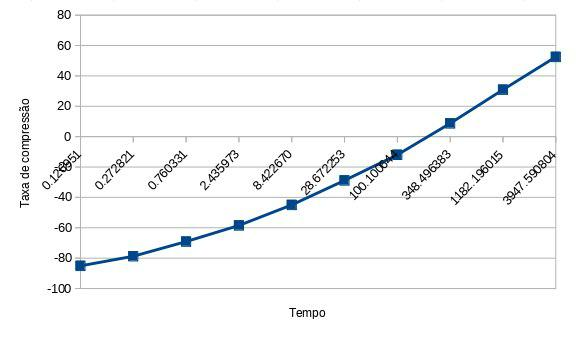
\includegraphics[width=7cm,height=4cm]{ASCII.jpg}\\
	Imagem 2 - Taxa de compressão x Tempo de execução para arquivo ASCII.
\end{center}

\begin{center}
	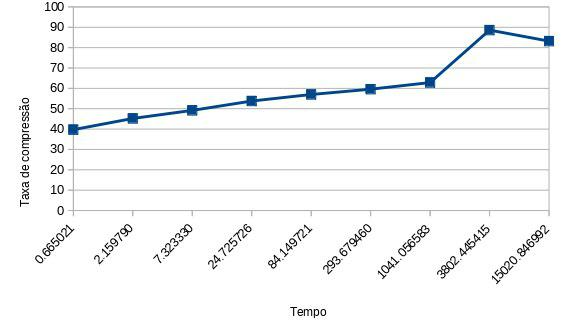
\includegraphics[width=7cm,height=4cm]{Binario.jpg}\\
	Imagem 3 - Taxa de compressão x Tempo de execução para arquivo binário.
\end{center}

Os gráficos mostram que a taxa de compressão de arquivos binários tende a ser maior que a de arquivos texto em formato ASCII. Comprimindo consideravalmente mais que os arquivos comuns de texto.

\subsection{Descompactação}
Após compactar todos os arquivos com sucesso, utilizou-se o algoritmo de descompactação para averiguar o tempo demandado e a veracidade dos dados originais. Com os resultados da descompactação de cada um dos 19 arquivos foi possível ver que os dados do arquivo de saída (o descompactado) eram exatamente iguais aos arquivos antes de serem compactados, mostrando a correta funcionalidade do algoritmo. Sendo assim foi possível gerar os gráficos de tempo, como mostrados abaixo:

\begin{center}
	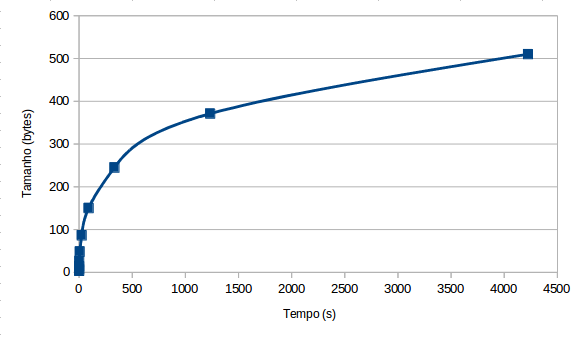
\includegraphics[width=7cm,height=4cm]{UNTXT.png}\\
	Imagem 4 - Tempo de execução x Taxa de descompactação para o arquivo texto normal.
\end{center}

Em que mostra o crescimento rápido do tempo de execução a medida que o tamanho do arquivo a ser compactado aumenta. Já no gráfico abaixo, para a descompactação do arquivo binário, observa-se que o tempo de execução aumenta rapidamente também, mas em contradição, o tamanho do arquivo de dicionário apresenta uma queda, confirmando que a partir de um determinado tamanho do dicionário, para arquivo binário, heverão várias repetições que se assemelharão a outras, diminuindo grandemente o tamanho final do arquivo de dicionário.

\begin{center}
	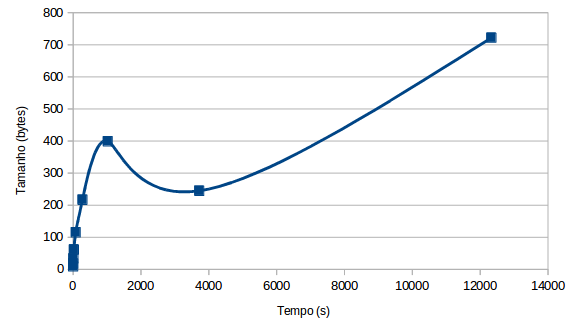
\includegraphics[width=7cm,height=4cm]{UNBIN.png}\\
	Imagem 5 - Tempo de execução x Taxa de descompactação para o arquivo binário.
\end{center}

\section{Conclusão}
Com a finalização do trabalho, foi possível notar que o algoritmo LZ78 possui uma alta capacidade de compactação, mas, por outro lado, possui uma taxa de crescimento de tempo de execução alta, tornando-se inviável para a compactação de arquivos maiores que 1,4MB para formato texto e 4,2MB para formato binário. Em consequência de não serem utilizadas nenhumas técnicas de diminuição do tamanho do dicionário, o seu algoritmo tende a ser mais demorado, ocupando mais espaço em disco. Com o decorrer das análises, pôde-se perceber também que arquivos com formato binário possuem uma maior capacidade de compactação comparados a arquivos de formato texto, por possuírem uma maior semelhança de caracteres no dicionário, não criando tantas duplas quanto necessário para o outro tipo de arquivo, mostrando que o algoritmo possui uma melhor compactação em imagens e arquivos .bin, tal como ZHAO e MUTHUSAMY \cite{muthusamy2012} afirmaram.

\bibliography{referencias}

\end{document}
